\documentclass[10pt,a4paper]{article}
\usepackage[dvipsnames]{xcolor}
\usepackage{booktabs}
\usepackage{amsmath}
\usepackage{graphicx}
\usepackage{multicol}
\usepackage{listings}
\usepackage{color}
\usepackage{float}
\usepackage[left=2cm,right=2cm,top=2cm,bottom=2cm]{geometry}

\begin{document}

\begin{titlepage}
	\centering
	{ \huge \scshape National Polytechnic Institute\par}
	{ \Large \scshape  Superior School of Computer Sciences\par }
	\vspace{1cm}
	{\scshape\Large Algorithm Analysis.\par}
	\vspace{1.5cm}
	{\Huge\bfseries Practice 1 - Experimental Determination of the Temporal Complexity of an Algorithm.\par}
	\vspace{2cm}
	{\Large\itshape Hernandez Martinez Carlos David.\par}
	{\Large\itshape davestring@outlook.com.\par}
	{\Large\itshape Group: 3cv2. \par}
	\vfill
	{\large \today\par} 
	\vfill
\end{titlepage}

\renewcommand\lstlistingname{Quelltext} 

\lstset{ 
	language=Python,
	basicstyle=\small\sffamily,
	numbers=left,
 	numberstyle=\tiny,
	frame=tb,
	tabsize=4,
	columns=fixed,
	showstringspaces=false,
	showtabs=false,
	keepspaces,
	commentstyle=\color{lightgray},
	keywordstyle=\color{Violet} \bfseries,
	stringstyle=\color{MidnightBlue}
}

\tableofcontents 
\pagenumbering {arabic}
\pagebreak

\section{Introduction:}

To say that a problem is solvable algorithmically means, informally, that a computer program
can be written that will produce the correct answer for any input if we let it run long
enough and allow it as much storage space as it needs. In the 1930s, before the advent of
computers, mathematicians worked very actively to formalize and study the notion of an
algorithm, which was then interpreted informally to mean a clearly specified set of simple
instructions to be followed to solve a problem or compute a function. Various formal
models of computation were devised and investigated. Much of the emphasis in the early
work in this field, called {\bfseries\itshape computability theory}, was on describing or characterizing those
problems that could be solved algorithmically and on exhibiting some problems that could
not be. One of the important negative results, established by Alan Turing, was the proof
of the unsolvability of the “halting problem.” The halting problem is to determine whether
an arbitrary given algorithm (or computer program) will eventually halt (rather than, say,
get into an infinite loop) while working on a given input. There cannot exist a computer
program that solves this problem. [ 1 ] \hfill \break

Although computability theory has obvious and fundamental implications for computer
science, the knowledge that a problem can theoretically be solved on a computer is not
sufficient to tell us whether it is practical to do so. For example, a perfect chess-playing
program could be written. This would not be a very difficult task; there are only a finite
number of ways to arrange the chess pieces on the board, and under certain rules a game
must terminate after a finite number of moves. The program could consider each of the
computer’s possible moves, each of its opponent’s possible responses, each of its possible
responses to those moves, and so on until each sequence of possible moves reaches an end.
Then since it knows the ultimate result of each move, the computer can choose the best
one. The number of distinct arrangements of pieces on the board that it is reasonable to
consider (much less the number of sequences of moves) is roughly 1050 by some estimates.
A program that examined them all would take several thousand years to run. Thus such a
program has not been run. [ 1 ] \hfill \break

Numerous problems with practical applications can be solved — that is, programs can
be written for them — but the time and storage requirements are much too great for these
programs to be of practical use. Clearly the time and space requirements of a program are
of practical importance. They have become, therefore, the subject of theoretical study in
the area of computer science called {\bfseries\itshape computational complexity}. [ 1 ]

\pagebreak

\section{Basic Concepts:}

\begin{itemize}
\item $\theta$ Notation:
\end{itemize} 
A $\theta$( g( n ) )  is defined as: \hfill \break

$\theta$ ( g( n ) ) = $\lbrace$ f( n ) $\mid$ $\exists$ $C_{1}$, $C_{2}$ $>$ 0 and $n_{0}$ $>$ 0 then 0 $\leq$ $C_{1}$g ( n ) $\leq$ f( n ) $\leq$ $C_{2}$g( n ) $\forall$ n $\geq$ $n_{0}$ $\rbrace$ \hfill \break

\begin{itemize}
\item O Notation:
\end{itemize} 
A O( g( n ) )  is defined as: \hfill \break

O ( g( n ) ) = $\lbrace$ f( n ) $\mid$ $\exists$ C, $n_{0}$ $>$ 0 then 0 $\leq$ f( n ) $\leq$ Cg( n ) $\forall$ n $\geq$ $n_{0}$ $\rbrace$ \hfill \break

\begin{itemize}
\item $\Omega$ Notation:
\end{itemize} 
A $\Omega$( g( n ) )  is defined as: \hfill \break

$\Omega$ ( g( n ) ) = $\lbrace$ f( n ) $\mid$ $\exists$ C, $n_{0}$ $>$ 0 then 0 $\leq$ g( n ) $\leq$ f( n ) $\forall$ n $\geq$ $n_{0}$ $\rbrace$ \hfill \break


\pagebreak

\section{Development:}

\subsection{Binary Sum:}

The program is divided in three python modules for have a better control of the code. 

\begin{itemize}
\item main.py: Contain the method "generate", "display" and "main".
\item graph.py: Evaluate {\bfseries{\itshape time}}  against {\bfseries{\itshape r=n}} where 'n' is the length of the binary number list.
\item binarysum.py: Contains the algorithm that implements the sum.
\end{itemize}

\subsubsection{Main.py}

In main.py there is a method named "generate" and will initialize and fill 2 lists of binary numbers generated randomly, of course, after having define the size of both lists. This sizes are of order {\bfseries{\itshape two to the power of 'n' ( $2^n$ )}}. Note that can be {\bfseries{\itshape n $>$ m}} or {\bfseries{\itshape n $=$ m}} but never {\bfseries{\itshape n $<$ m}}. This because the {\bfseries{\itshape for}} in the line 10 it's from {\bfseries{\itshape i = 0 }} to {\bfseries{\itshape 'n'}}, this means that the size of the lists {\bfseries{\itshape 'a'}} and {\bfseries{\itshape 'b'}} are both of size {\bfseries{\itshape 'n'}}. In case that {\bfseries{\itshape n $>$ m}} the rest of the list {\bfseries{\itshape 'b'}} will be filled with {\bfseries{\itshape 0's}}. \hfill \break

\begin{lstlisting}
def generate ( ):
    a, b, n, m = [ ], [ ], 0, 1
    # Define the size of a-b lists ( n-m respectively ).
    while ( n < m ):
        rnd = ( int ( random ( ) * 5 ) + 1 )
        n = int ( pow ( 2, rnd ) )
        rnd = ( int ( random ( ) * 5 ) + 1 )
        m = int ( pow ( 2, rnd ) )
    # Generate both binary numbers as integer lists.
    for i in range ( n ):
        a.insert ( 0, ( ( int ( random ( ) * 2 ) + 0 ) ) )
        if ( i >= m ):
            b.insert ( 0, 0 )
        else:
            b.insert ( 0, ( ( int ( random ( ) * 2 ) + 0 ) ) )
    # Return statement.
    return a, b
\end{lstlisting} \hfill 

The method "display" it's more simple, its only function it's to display in console the binary numbers ( lists ) {\bfseries{\itshape a [ n ]}} and {\bfseries{\itshape b [ n ]}}, the result of the sum stored in a list {\bfseries{\itshape 'c'}} and the order of the resulting list ( $2^p$ ) as the figure 4.1.0 shows. \hfill \break

\begin{lstlisting}
def display ( a, b, c ):
    DATAFORMAT = ""
    if ( len ( c ) > len ( a ) ): DATAFORMAT = "   "
    print ( "\n\tA: " + DATAFORMAT, a )
    print ( "\tB: " + DATAFORMAT, b )
    print ( "\tC: ", c )
    print ( "\n\tOrder of the sum: ", int ( pow ( 2, len ( c ) - 1 ) ), "\n" )
\end{lstlisting} \hfill

Finally, the method "main", aside of being the principal, calls the others methods and controls the sequence of execution. \hfill  \break

\begin{lstlisting}
def main ( ):
    a, b = generate ( )
    c = binarysum ( a, b )
    display ( a, b, c )
main ( )
\end{lstlisting}

\pagebreak

\subsubsection{Binarysum.py}

Principal module, contains the algorithm that we are determining the temporal complexity. As the binary sum works, the code takes the values of the {\bfseries{\itshape n - i}} positions, and evaluates: 

\begin{itemize}
\item With carry = 0:
\begin{enumerate}
\item If {\bfseries\textcolor{Blue}{0}} + 0 + 0 = 00 then {\bfseries{\itshape sum = 0}} and {\bfseries{\itshape carry = 0}}.
\item If {\bfseries\textcolor{Blue}{0}} + 0 + 1 = 01 then {\bfseries{\itshape sum = 1}} and {\bfseries{\itshape carry = 0}}.
\item If {\bfseries\textcolor{Blue}{0}} + 1 + 0 = 01 then {\bfseries{\itshape sum = 1}} and {\bfseries{\itshape carry = 0}}.
\item If {\bfseries\textcolor{Blue}{0}} + 1 + 1 = 10 then {\bfseries{\itshape sum = 0}} and {\bfseries{\itshape carry = 1}}.
\end{enumerate}
\item With carry = 1:
\begin{enumerate}
\item If {\bfseries\textcolor{Blue}{1}} + 0 + 0 = 01 then {\bfseries{\itshape sum = 1}} and {\bfseries{\itshape carry = 0}}.
\item If {\bfseries\textcolor{Blue}{1}} + 1 + 0 = 10 then {\bfseries{\itshape sum = 0}} and {\bfseries{\itshape carry = 1}}.
\item If {\bfseries\textcolor{Blue}{1}} + 0 + 1 = 10 then {\bfseries{\itshape sum = 0}} and {\bfseries{\itshape carry = 1}}.
\item If {\bfseries\textcolor{Blue}{1}} + 1 + 1 = 11 then {\bfseries{\itshape sum = 1}} and {\bfseries{\itshape carry = 1}}.
\end{enumerate}
\end{itemize}

... So on, until reaching the numbers of the 0 position. In case of {\bfseries{\itshape carry = 1}}, a '1' is added to the position {\bfseries{\itshape c [ 0 ]}}. of the list, as the line 20 shows. \hfill \break

\begin{lstlisting}
def binarysum ( a, b ):
    i, carry, c = ( len ( a ) - 1 ), 0, [ ]
    # Evaluate both binary lists ( 'a' and 'b' ) and scroll through from ( n - 1 ) to 0
    # and sum the numbers at 'i' position, the result is stored in 'c'.
    while ( i >= 0 ):
        if ( ( a [ i ] + b [ i ] + carry ) == 1 ):
            c.insert ( 0, 1 )
            carry = 0
        elif ( ( a [ i ] + b [ i ] + carry ) == 2 ):
            c.insert ( 0, 0 )
            carry = 1
        elif ( ( a [ i ] + b [ i ] + carry ) == 3 ):
            c.insert ( 0, 1 )
            carry = 1
        else:
            c.insert ( 0, 0 )
            carry = 0
        i = i - 1
    # After finish, evaluates if there is a carry value.
    if ( carry == 1 ):
        c.insert ( 0, carry )
    # Return statement.
    return c
\end{lstlisting}

{\bfseries{\itshape Observation:}} {\itshape Because it is a list, elements can easily be inserted or removed without reallocation or reorganization of the entire structure.} \hfill \break

\pagebreak

To analyze the temporal complexity of the algorithm it's necessary to put a counter in each line of the code, this line will help to plot {\bfseries\itshape time ( t )} against {\bfseries\itshape size ( n )}. \hfill \break

\begin{lstlisting}
def binarysum ( a, b ):
    i, carry, c, count = ( len ( a ) - 1 ), 0, [ ], 1
    # Evaluate both binary lists ( 'a' and 'b' ) and scroll through from ( n - 1 ) to 0
    # and sum the numbers at 'i' position, the result is stored in 'c'.
    while ( i >= 0 ):
        count += 1
        if ( ( a [ i ] + b [ i ] + carry ) == 1 ):
            count += 1
            c.insert ( 0, 1 )
            count += 1
            carry = 0
            count += 1
        elif ( ( a [ i ] + b [ i ] + carry ) == 2 ):
            count += 1
            c.insert ( 0, 0 )
            count += 1
            carry = 1
            count += 1
        elif ( ( a [ i ] + b [ i ] + carry ) == 3 ):
            count += 1
            c.insert ( 0, 1 )
            count += 1
            carry = 1
            count += 1
        else:
            count += 1
            c.insert ( 0, 0 )
            count += 1
            carry = 0
            count += 1
        i = i - 1
        count += 1
    count += 1
    # After finish, evaluates if there is a carry value.
    count += 1
    if ( carry == 1 ):
        c.insert ( 0, carry )
        count += 1
    # Return statement.
    return c, count
\end{lstlisting} 
{\bfseries\itshape Observation:} {\itshape Note that the return statement it's the counter and the result of the sum stored in a list, were the counter will be the vertical axis and the length of 'c' the horizontal axis.} \hfill \break

\pagebreak

\subsubsection{Graph.py}

For plotting the result I'm using two python tools named {\bfseries\itshape matplotlib.pyplot} and {\bfseries\itshape numpy}. The module {\bfseries\itshape graph.py} has two methods. The first one is {\bfseries\itshape parameters ( )}. This method create the points where the curve will be plotted according to the parameters that {\bfseries\itshape main} sends. \hfill \break

\begin{lstlisting}
def parameters ( size, time ):
    # time vs size graph points.
    t, n = [ ], [ 0 ]
    # div: Auxiliar variable that help to plot the graph.
    div = float ( "{0:.2f}".format ( 1 / round ( time / size ) ) )
    # Time ( t ) parameters.
    for i in range ( time ):
        t.append ( i )
    # Size ( n ) parameters.
    for i in range ( time ):
        if ( i != 0 ):
            n.append ( float ( "{0:.2f}".format ( n [ i - 1 ] + div ) ) )
    # Return statement.
    return t, n
\end{lstlisting} \hfill 

Finally the last method is {\bfseries\itshape graph ( )}, as the name says, plot the graphic of the temporal complexity for this algorithm comparing {\bfseries\itshape time ( t )} against {\bfseries\itshape size ( n )}. \hfill \break

\begin{lstlisting}
def graph ( size, time ):
    # Window title.
    plt.figure ( "Temporal Complexity of Binary Sum Algorithm" )
    # Graph title.
    plt.title ( "Binary Sum:", color = ( 0.3, 0.4, 0.6 ), weight = "bold" )
    # Construct the parameters of the graph.
    t, n = parameters ( size, time )
    # Define the limits of the graph.
    plt.xlim ( 0, size )
    plt.ylim ( 0, time )
    # Proposed function: g ( n ) = ( 3/2 )n.
    _t = list ( map ( ( lambda x: x * 3/2 ), t ) )
    # Names of the axes.
    plt.xlabel ( "Size ( n )", color = ( 0.3, 0.4, 0.6 ), 
    	family = "cursive", size = "large" )
    plt.ylabel ( "Time ( t )", color = ( 0.3, 0.4, 0.6 ), 
    	family = "cursive", size = "large" )
    # Plot.
    plt.plot ( n, _t, "#800000", linestyle = "--", label = "g( n ) = ( 3/2 )n" )
    plt.plot ( n, t, "#778899", linewidth = 3, label = "E( n ) = n" )
    plt.legend ( loc = "lower right" )
    plt.show ( )
\end{lstlisting} \hfill \break

\pagebreak

\subsection{Euclidean Algorithm:}

The program is divided in four python modules for have a better control of the code. 

\begin{itemize}
\item main.py: Contain the method "generate", "display", "menu" and "main".
\item graph.py: Evaluate {\bfseries{\itshape time}}  against {\bfseries{\itshape gcd}} where gcd it's the gratest common divisor of 'n' and 'm'.
\item euclidean.py: Contains the Euclidean Algorithm.
\item fibonacci.py: Return a list of 'n' Fibonacci numbers.
\end{itemize}

\subsubsection{Main.py}

In main.py there is a {\bfseries\itshape menu ( )} method, the user will have two options, generate random numbers or use the Fibonacci numbers to calculate their GCD using the Euclidean algorithm. In case that the user chose for random numbers, {\bfseries\itshape main ( )} will call the method generate and will return two numbers, {\bfseries\itshape 'n' and 'm'}. \hfill \break

\begin{lstlisting}
def generate ( ):
    n, m = 0, 1
    while ( n < m ):
        n = ( int ( random ( ) * 1000 ) + 1 )
        m = ( int ( random ( ) * 1000 ) + 1 )
    # Return statement.
    return n, m
\end{lstlisting} \hfill

... In other case, {\bfseries\itshape main ( )} will call {\bfseries\itshape fibonacci ( )} ( see section 3.2.2 ). As we can see, the principal work of this method is to control the execution sequence of the program. \hfill \break

\begin{lstlisting}
def main ( ):
    ans = menu ( )
    if ( ans == 2 ):
        print ( "\n\tFirst 'n' Fibonacci's to calculate: " )
        limit = int ( input ( "\tAnswer: " ) )
        # Return a Fibonacci numbers list.
        fibo = fibolist ( limit )
        # Assign the last two Fibonacci's in the list.
        n, m = fibo [ len ( fibo ) - 1 ], fibo [ len ( fibo ) - 2 ]
    else:
        # Generate random numbers.
        n, m = generate ( )
    # Return: GCD, algorithm counter for temporal complexity and gcd process list.
    result, count, gcd = algorithm ( n, m )
    # Display on screen the result.
    display ( n, m, result )
    # Graph of the Temporal Complexity of the Euclidean Algorithm.
    graph ( n, m, count, gcd )

main ( )
\end{lstlisting} 

\pagebreak

\subsubsection{Fibonacci.py}

The module has two methods {\bfseries\itshape fibonacci ( )} and {\bfseries\itshape fibolist ( )}. The first method create a generator of Fibonacci numbers, and the second method returns a 'list' of the firsts 'n' Fibonacci numbers. \hfill \break

\begin{lstlisting}
# Fibonacci Generator.
def fibonacci ( ):
    a, b = 1, 1
    while ( True ):
        yield a
        a, b = b, a + b
\end{lstlisting} \hfill 

The program call {\bfseries\itshape fibonacci ( )} in line '5' inside a {\bfseries\itshape for} loop, this because the method it's a generator. \hfill \break

\begin{lstlisting}
# Fibonacci list.
def fibolist ( limit ):
    n, fibo = 0, [ ]
    # Create a Fibonacci numbers list using a generator.
    for i in fibonacci ( ):
        if ( n >= limit ): break
        fibo.append ( i )
        n += 1
    # Return statement.
    return fibo
        a, b = b, a + b
\end{lstlisting}

{\bfseries\itshape Observation:} {\itshape Note that fibolist ( ) receive as parameter a 'limit', this integer will define to which number we want the generator to calculate.}

\pagebreak

\subsubsection{Euclidean.py}

The principal module, contains the algorithm that we are determining the temporal complexity. The Euclidean algorithm proceeds in a series of steps such that the output of each step is used as an input for the next one. Let {\bfseries\itshape k} be an integer that counts the steps of the algorithm, starting with zero. Thus, the initial step corresponds to {\bfseries\itshape k = 0}, the next step corresponds to {\bfseries\itshape k = 1}, and so on. \hfil \break

Each step begins with two non-negative remainders {\bfseries\itshape r$_{k-1}$} and {\bfseries\itshape r$_{k-2}$} Since the algorithm ensures that the remainders decrease steadily with every step, {\bfseries\itshape r$_{k-1}$} is less than its predecessor {\bfseries\itshape r$_{k-2}$}. The goal of the {\bfseries\itshape k}th step is to find a quotient {\bfseries\itshape q$_{k}$} and remainder {\bfseries\itshape r$_{k}$} that satisfy the equation

\begin{equation}
r_{k-1} = q_{k}r_{k-1} + r_{k}
\end{equation}

and that have {\bfseries\itshape r$_{k}$} $<$ {\bfseries\itshape r$_{k-1}$}. In other words, multiples of the smaller number {\bfseries\itshape r$_{k-1}$} are subtracted from the larger number {\bfseries\itshape r$_{k-2}$} until the remainder{\bfseries\itshape r$_{k}$} is smaller than {\bfseries\itshape r$_{k-1}$}. The implementation can be the following one. \hfill \break

\begin{lstlisting}
def algorithm ( n, m ):
    # Euclidean algorithm: Find the Greatest Common Divisor ( gcd ).
    while ( m != 0 ):
        r = n % m
        n = m
        m = r
    # return statement.
    return n
\end{lstlisting} \hfill 

The program return the Greatest Common Divisor, but to determinate the time that the algorithm takes to find the GCD we need to use a counter in each line of the code, and later compare it with the parameter {\bfseries\itshape 'n'}. \hfill \break

{\bfseries\itshape Observation:} {\itshape Parameter 'n' always will be bigger than 'm'.}. \hfill \break

\begin{lstlisting}
def algorithm ( n, m ):
    # Euclidean algorithm: Find the Greatest Common Divisor ( gcd ).
    count, gcd = 1, [ ]
    while ( m != 0 ):
        gcd.append ( n )
        count += 1
        r = n % m
        count += 1
        n = m
        count += 1
        m = r
        count += 1
    count += 1
    # return statement.
    return n, count, gcd
\end{lstlisting} \hfill 

{\bfseries\itshape Observation:} {\itshape Now apart of returning the GCD, returns the counter, and the list of the Euclidean process.}

\pagebreak

\subsubsection{Graph.py}
 
For plotting the result I'm using {\bfseries\itshape matplotlib} and {\bfseries\itshape numpy} and comparing the {\bfseries\itshape time ( t )} determined by the counter and the 'list' of the GCD Euclidean process created in the module {\bfseries\itshape euclidean.py}. The program is able to plot the curve of the temporal complexity of the algorithm. \hfill \break

\begin{lstlisting}
def graph ( n, m, count, gcd ):
    # Window title.
    plt.figure ( "Temporal Complexity of Euclidean Algorithm" )
    # Graph title.
    plt.title ( "Euclidean ( " + str ( n ) + ", " + str ( m ) + " ):", 
    	color = ( 0.3, 0.4, 0.6 ), weight = "bold" )
    # Parameter Time ( t ) of the graph.
    t = np.arange ( 0, count, ( count / len ( gcd ) ) )
    # Parameter Euclidean ( n ) of the list
    gcd.reverse ( )
    # Names of the axes.
    plt.xlabel ( "Euclidean ( e )", color = ( 0.3, 0.4, 0.6 ), 
    	family = "cursive", size = "large" )
    plt.ylabel ( "Time ( t )", color = ( 0.3, 0.4, 0.6 ), 
    	family = "cursive", size = "large" )
    # Proposed function: g ( n ) = ( 3/2 ) log ( n ).
    _t = list ( map ( ( lambda x: x * ( 3 / 2 ) ), t ) )
    # Plot.
    plt.plot ( gcd, _t, "#800000", linestyle = "--", 
    	label = "g( n ) = ( 3/2 ) log ( n )" )
    plt.plot ( gcd, t, "#778899", linewidth = 3, 
    	label = "E( n ) = log ( n )" )
    plt.legend ( loc = "lower right" )
    plt.show ( )
\end{lstlisting}
\pagebreak

\section{Results:}

All the code shown above doesn't have significance if its operation is not shown. This section will show you the {\bfseries\itshape console} output and the graphic of the temporal complexity of the algorithms previously mentioned.

\subsection{Binary Sum Algorithm:}

First test of the binary sum between 'A' and 'B', the result is stored in 'C'.

\begin{figure}[H]
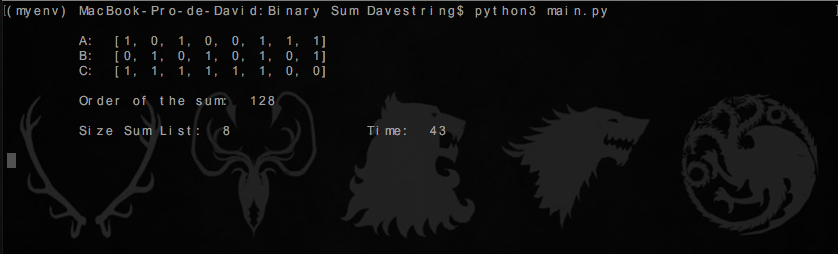
\includegraphics[scale=.6]{result1.png}
\centering \linebreak \linebreak Figure 4.1.0: Binary sum result.
\end{figure}

\begin{multicols}{2}
\begin{figure}[H]
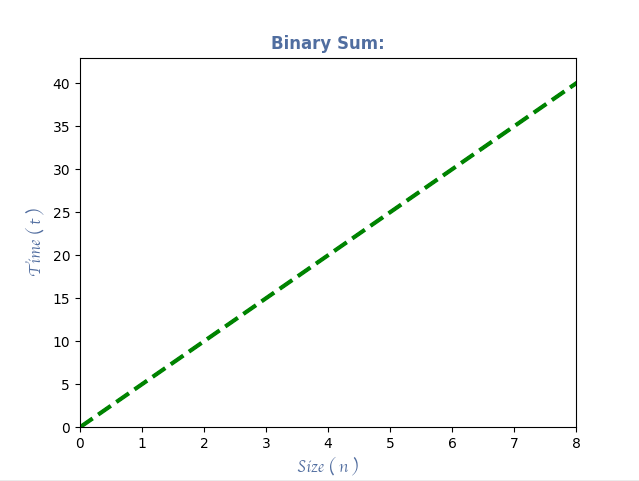
\includegraphics[scale=.4]{graph1.png}
\centering \linebreak \linebreak Figure 4.1.1: Plot of the Binary sum of figure 4.1.0.
\end{figure}
\hfill \break

{\bfseries\itshape Observation:} {\itshape In figure 4.1.0 the shell display the time that the algorithm take to finish and the size of the resulting list, in the graph ( figure 4.1.1 ) those are the range of the axes.}
\end{multicols}

\pagebreak

Second test of the binary sum between 'A' and 'B', the result is stored in 'C'.

\begin{figure}[H]
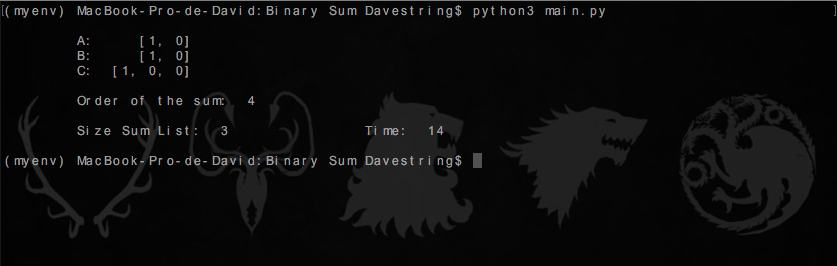
\includegraphics[scale=.6]{result2.png}
\centering \linebreak \linebreak Figure 4.1.2: Binary sum result.
\end{figure}

\begin{multicols}{2}
\begin{figure}[H]
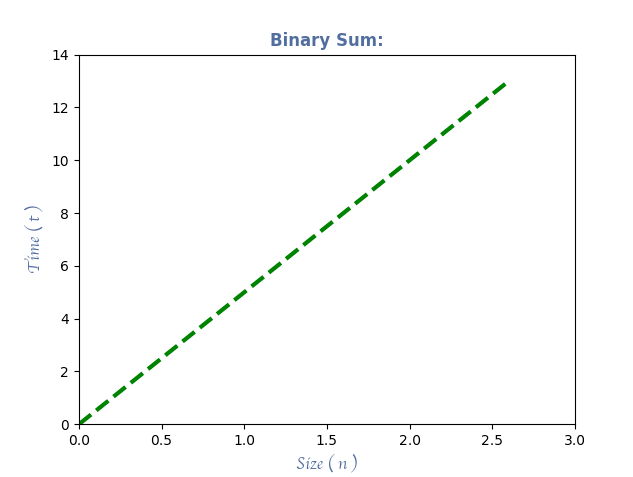
\includegraphics[scale=.4]{graph2.png}
\centering \linebreak \linebreak Figure 4.1.3: Plot of the Binary sum of figure 4.1.2.
\end{figure}
\hfill \break

\begin{center}
\begin{tabular}[.5cm]{l c c }
\toprule
time ( t ) & size ( n ) \\
\midrule
0 & 0 \\
\cmidrule{1-2}
1 & 0.2 \\
\cmidrule{1-2}
2 & 0.4 \\
\cmidrule{1-2}
3 & 0.6 \\
\cmidrule{1-2}
4 & 0.8 \\
\cmidrule{1-2}
5 & 1.0 \\
\cmidrule{1-2}
6 & 1.2 \\
\cmidrule{1-2}
7 & 1.4 \\
\cmidrule{1-2}
8 & 1.6 \\
\cmidrule{1-2}
9 & 1.8 \\
\cmidrule{1-2}
10 & 2.0 \\
\cmidrule{1-2}
11 & 2.2 \\
\cmidrule{1-2}
12 & 2.4 \\
\cmidrule{1-2}
13 & 2.6 \\
\bottomrule
\linebreak
\end{tabular}
\centering \linebreak \linebreak Table 4.1.0: Plot points of figure 4.1.3.
\end{center}
\end{multicols}

\pagebreak

\subsection{Euclidean Algorithm:}

First we are going to analyze the worst case for this algorithm, and it's when the entry are Fibonacci numbers. The result will be of {\bfseries\itshape logarithmic} order.

\begin{figure}[H]
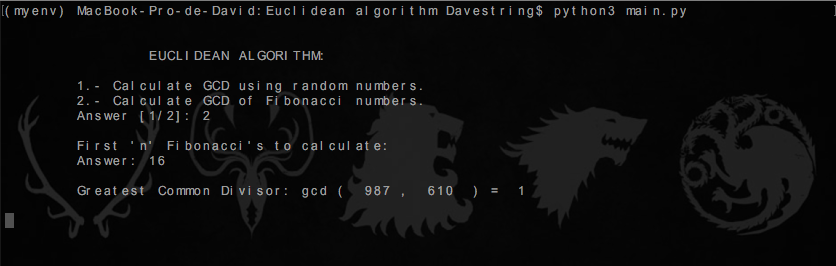
\includegraphics[scale=.6]{fibo1.png}
\centering \linebreak \linebreak Figure 4.2.0: Greatest Common Divider of 2 Fibonacci Numbers.
\end{figure}

\begin{figure}[H]
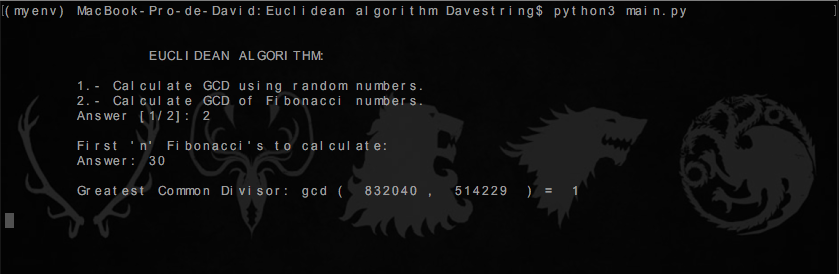
\includegraphics[scale=.6]{fibo2.png}
\centering \linebreak \linebreak Figure 4.2.1: Greatest Common Divider of 2 Fibonacci Numbers.
\end{figure}

\begin{multicols}{2}
\begin{figure}[H]
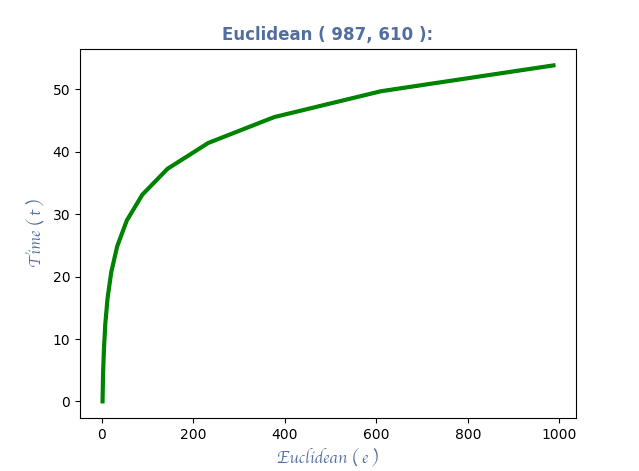
\includegraphics[scale=.4]{fibograph1.png}
\centering \linebreak \linebreak Figure 4.2.2: Plot of time ( t ) against euclidean ( e ) of Figure 4.2.0.
\end{figure}

\begin{figure}[H]
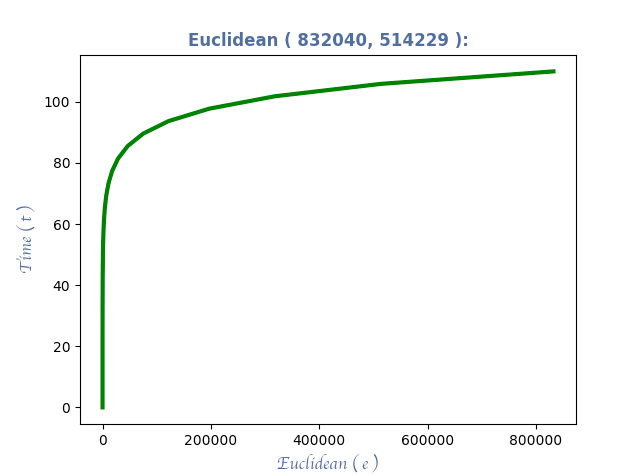
\includegraphics[scale=.4]{fibograph2.png}
\centering \linebreak \linebreak Figure 4.2.3: Plot of time ( t ) against euclidean ( e ) of Figure 4.2.1.
\end{figure}
\end{multicols} \pagebreak

This other cases are basically two numbers generated randomly. They may can take a {\bfseries\itshape logarithmic} form or not because of the plotting points, but still of {\bfseries\itshape logarithmic} order.

\begin{figure}[H]
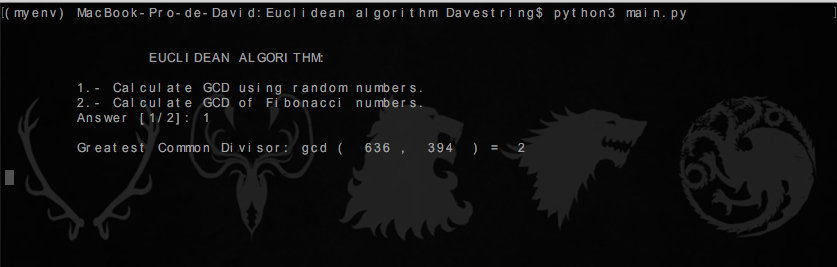
\includegraphics[scale=.6]{result3.png}
\centering \linebreak \linebreak Figure 4.2.4: Greatest Common Divider of 2 Random Numbers.
\end{figure}

\begin{figure}[H]
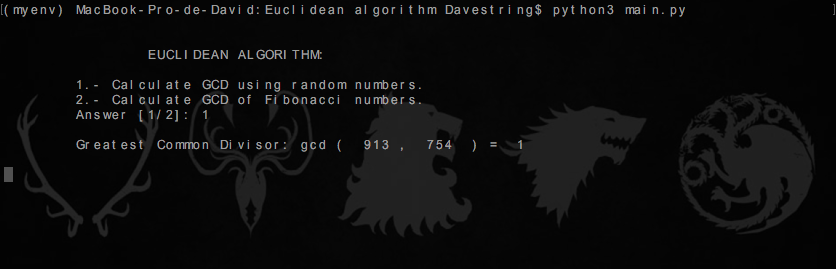
\includegraphics[scale=.6]{result4.png}
\centering \linebreak \linebreak Figure 4.2.5: Greatest Common Divider of 2 Random Numbers.
\end{figure}

\begin{multicols}{2}
\begin{figure}[H]
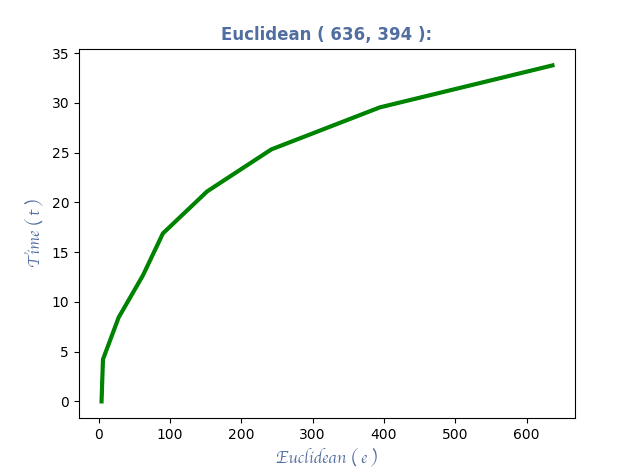
\includegraphics[scale=.4]{graph3.png}
\centering \linebreak \linebreak Figure 4.2.6: Plot of time ( t ) against euclidean ( e ) of Figure 4.2.4.
\end{figure}

\begin{figure}[H]
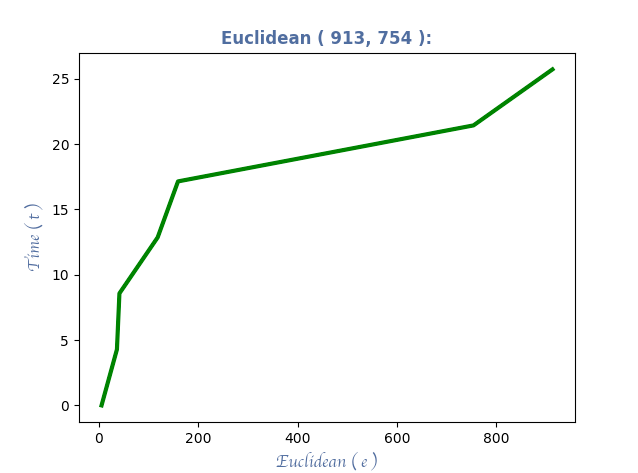
\includegraphics[scale=.4]{graph4.png}
\centering \linebreak \linebreak Figure 4.2.7: Plot of time ( t ) against euclidean ( e ) of Figure 4.2.5.
\end{figure}
\end{multicols} \pagebreak

\subsubsection{Plot Tables:}

The following tables are the points with which the graphs of the Euclidean Algorithm were plotted. I didn't put the other tables because there were too many points.
	
\begin{multicols}{2}
\begin{center}
\begin{itemize}
\item Euclidean ( 987, 610 ):
\end{itemize}  \hfill \break
\begin{tabular}[.5cm]{l c c }
\toprule
euclidean ( e ) & time ( t )  \\
\midrule
2 & 0 \\
\cmidrule{1-2}
3 & 4.14 \\
\cmidrule{1-2}
5 & 8.28 \\
\cmidrule{1-2}
8 & 12.42 \\
\cmidrule{1-2}
13 & 16.57 \\
\cmidrule{1-2}
21 & 20.71 \\
\cmidrule{1-2}
34 & 24.85 \\
\cmidrule{1-2}
55 & 29 \\
\cmidrule{1-2}
89 & 33.14 \\
\cmidrule{1-2}
144 & 37.28 \\
\cmidrule{1-2}
233 & 41.42 \\
\cmidrule{1-2}
377 & 45.57 \\
\cmidrule{1-2}
610 & 49.71\\
\cmidrule{1-2}
987 & 53.85 \\
\bottomrule
& \\
Table 4.2.1.0: Plot points of figure 4.2.2.
\end{tabular}
\end{center}

\begin{center}
\begin{itemize}
\item Euclidean ( 913, 754 ):
\end{itemize} \hfill \break
\begin{tabular}[.5cm]{l c c }
\toprule
euclidean ( e ) & time ( t )  \\
\midrule
5 & 0 \\
\cmidrule{1-2}
36 & 4.28 \\
\cmidrule{1-2}
41 & 8.57 \\
\cmidrule{1-2}
118 & 12.85 \\
\cmidrule{1-2}
159 & 17.14 \\
\cmidrule{1-2}
754 & 21.42 \\
\cmidrule{1-2}
913 & 25.71 \\
\bottomrule
\linebreak
\end{tabular}
\centering \linebreak \linebreak Table 4.2.1.1: Plot points of figure 4.2.7.
\end{center}
\end{multicols} 

\pagebreak

\subsection{Proposed Functions:}

For each Algorithm I propose a function {\bfseries\itshape g( n )} that satisfy the following requirements: 

\begin{itemize}
\item {\bfseries\itshape g( n )} and {\bfseries\itshape h( n )} are different for each algorithm.
\item {\bfseries\itshape g( n )} such that {\bfseries\itshape ( binarysum, euclidean )} $\in$ {\bfseries\itshape O( g( n ) )}.
\item if {\bfseries\itshape ( binarysum, euclidean )} $\in$ {\bfseries\itshape O( h( n ) )} then {\bfseries\itshape g( n )} $\in$ {\bfseries\itshape O( h( n ) )}
\end{itemize}

\subsubsection{Binary Sum g( n ):}

The binary sum algorithm is of {\bfseries\itshape linear} order. The function that I propose is {\bfseries\itshape g( n ) = $\frac{3}{2}$ n}.

\begin{figure}[H]
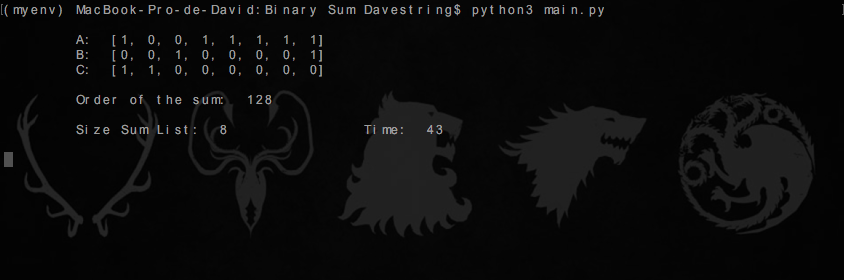
\includegraphics[scale=.6]{proposed1.png}
\centering \linebreak \linebreak Figure 4.3.1.0: Binary sum output.
\end{figure}

\begin{figure}[H]
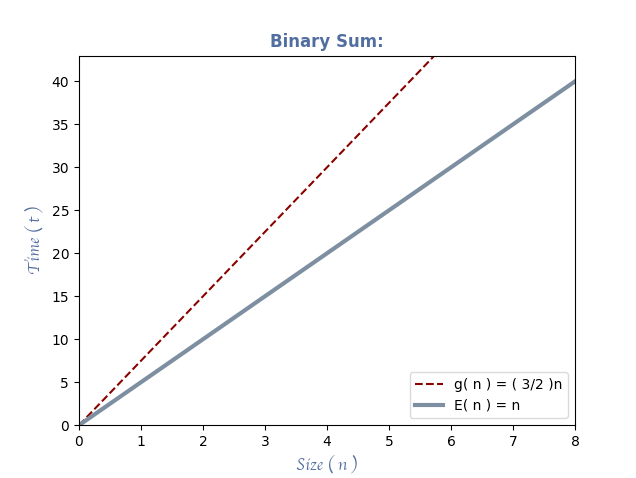
\includegraphics[scale=.6]{pgraph1.png}
\centering \linebreak \linebreak Figure 4.3.1.1: Binary sum proposed function plot.
\end{figure}

\pagebreak

\subsubsection{Euclidean Algorithm g( n ):}

The Euclidean algorithm is of {\bfseries\itshape logarithmic} order. The function that I propose is {\bfseries\itshape g( n ) = $\frac{3}{2}$ log( n )}.

\begin{figure}[H]
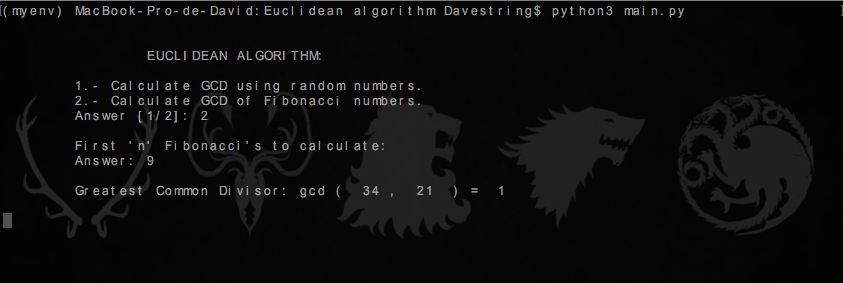
\includegraphics[scale=.6]{proposed2.png}
\centering \linebreak \linebreak Figure 4.3.2.0: Euclidean Algorithm output.
\end{figure}

\begin{figure}[H]
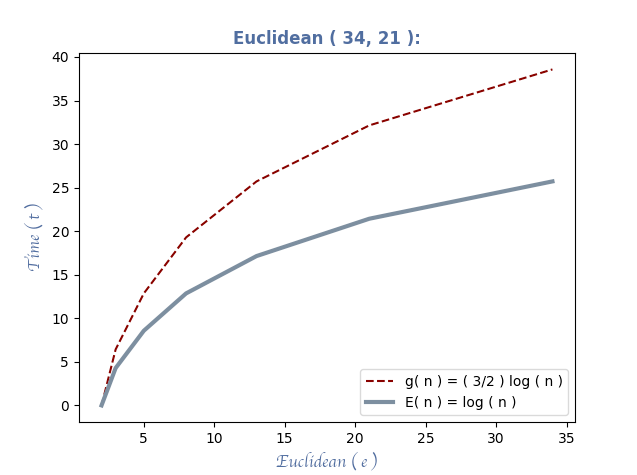
\includegraphics[scale=.6]{pgraph2.png}
\centering \linebreak \linebreak Figure 4.3.2.1: Euclidean proposed function plot.
\end{figure}

\pagebreak

\section{Conclusion:}

Always it's very interesting lead the theory to the practice, compute an algorithm and calculate the temporal complexity it's very different than doing it using all the theorems and definitions, but still very important to know what we are doing. Also, plotting result for me an interesting part, most with the {\bfseries\itshape Euclidean Algorithm}, I didn't expected that the GCD of a Fibonacci number where a sequence of the previous Fibonacci numbers, maybe I didn't stand to think on it a long time and it was obvious, but still, were a surprise for me. I actually have fun using {\bfseries\itshape matplotlib} and {\bfseries\itshape numpy}, python never stops surprising me with all the implemented stuff that has. \hfill \break

\pagebreak

\section{Annexes:}

Calculate the temporal complexity of the following algorithm:

\begin{lstlisting}
for ( i = 0 ) to i <= ( n - 2 ) do
	k = i
	for ( j = i + 1 ) to j >= ( n - 1 ) do
		if ( A [ j ] < A [ k ] ) then 
			k = j
	exchange ( A [ i ], A [ k ] )
\end{lstlisting}

Solution:

\begin{equation}
T ( n ) = C_{1}( n ) + C_{2}( n- 1) + C_{3} ( \sum_{j = 0}^{n - 2} ( t_{i} ) + C_{4} ( \sum_{j = 0}^{n - 2} ( t_{i - 1} ) + C_{5} ( \sum_{j = 0}^{n - 2 } ( t_{i - 1} ) + C_{6} 
\end{equation}

\begin{itemize}
\item $t_{i}$ calculated table:
\end{itemize}

\begin{center}
\begin{tabular}[.5cm]{l c c c }
\toprule
i & $t_{i}$ & range \\
\midrule
0 & n & 1 $<$ j $<$ n \\
\cmidrule{1-3}
1& n - 1 & 2 $<$ j $<$ n \\
\cmidrule{1-3}
2 & n - 2 & 3 $<$ j $<$ n \\
\cmidrule{1-3}
- & then & - \\
\cmidrule{1-3}
i & n - i & i $<$ j $<$ n \\
\bottomrule
\linebreak
\end{tabular}
\end{center} 

{\tiny
\begin{equation}
\begin{split}
T ( n ) &= C_{1}(n) + C_{2}( n - 1 ) + C_{3}[ \sum_{j=0}^{n-2}( n - i ) ] + C_{4}[ \sum_{j=0}^{n-2}( n - i - 1) ]  + C_{5}[ \sum_{j=0}^{n-2}( n - i - 1) ] + C_{6} \\
&= C_{1}(n) + C_{2}( n - 1 ) + C_{3}[ \sum_{j=0}^{n-2}( n ) ] - C_{3}[ \sum_{j=0}^{n-2}( i ) ] + C_{4}[ \sum_{j=0}^{n-2}( n ) ] -  C_{4}[ \sum_{j=0}^{n-2}( i ) ] -  C_{4}[ \sum_{j=0}^{n-2}( 1 ) ] + C_{5}[ \sum_{j=0}^{n-2}( n ) ] -  C_{5}[ \sum_{j=0}^{n-2}( i ) ] -  C_{5}[ \sum_{j=0}^{n-2}( 1 ) ] + C_{6} \\
&= C_{1}(n) + C_{2}( n - 1 ) + C_{3}(n)(n-1) - C_{3}\frac{(n-1)(n-2)}{2} + C_{4}(n)(n-1) - C_{4}\frac{(n-1)(n-2)}{2} - C_{4}(n-1) + C_{5}(n)(n-1) - C_{5}\frac{(n-1)(n-2)}{2} - C_{5}(n-1) + C_{6} \\
&= C_{1}(n) + C_{2}(n) + - C_{2} + C_{3}(n^{2}) - C_{3}(n) - C_{3}(\frac{n^{2}-3n+2}{2}) + C_{4}(n^{2}) - C_{4}(n) - C_{4}(\frac{n^{2}-3n+2}{2}) - C_{4}(n) + C_{4} + C_{5}(n^{2}) - C_{5}(n) - C_{5}(\frac{n^{2}-3n+2}{2}) \\
&- C_{5}(n) + C_{5} + C_{6} \\
&= (n^{2})[ C_{3} + C_{4} + C_{5}  - C_{3}(\frac{1}{2}) - C_{4}(\frac{1}{2}) - C_{5}(\frac{1}{2}) ]  + ( n ) [ C_{1} + C_{2} - C_{3} - 2C_{4} - 2C_{5} + C_{3}(\frac{3}{2}) + C_{4}(\frac{3}{2}) + C_{5}(\frac{3}{2}) ] + [ - C_{2}  + C_{4}  + C_{5} + C_{6}  - C_{3}  - C_{4}  - C_{5}] \\
&= (n^{2})[ C_{3}(\frac{1}{2}) + C_{4}(\frac{1}{2}) + C_{5}(\frac{1}{2}) ]  + ( n ) [ C_{1} + C_{2} + C_{3}(\frac{1}{2}) - C_{4}(\frac{1}{2}) - C_{5}(\frac{1}{2}) ] + [ - C_{2} + C_{6}  - C_{3} ] 
\end{split}
\end{equation}}
Finally: 
\begin{equation}
\begin{split}
T(n) = an^{2} + b(n) + c \Longrightarrow T(n) \in \theta (n^{2})
\end{split}
\end{equation}
\pagebreak

\section{Bibliography References:}

[ 1 ] Baase and Van Gelder. "Computer Algorithms: Introduction to Design and Analysis". Addison-Wesley.

\end{document}